\section{Our Approach}
Our objective in this paper is to propose a method the target type identification task that requires minimal effort for feature engineering.  We cast the type identification problem into regression problem and predict the relevance score of a type, given a query-entity pair.
Following the idea of TC and EC methods introduced in sections \ref{TC} and \ref{EC}, we define two type-centric $I_{TC}$ and entity-centric $I_{EC}$ matrices.  In the following we explain each of these matrices.%that models word level similarities via word embeddings. 



\boldsymbol{$I_{TC}$} \textbf{matrix:} For a given query-type pair $(q,t)$, we first extract top-K words representing type $t$. In order to extract these words, we concatenate all abstracts of entities associated with that type and make a pseudo document for each type. We then calculate the tf.idf score for all terms of these pseudo documents, and sort the words each  pseudo document based on their tf.idf score. Once the representative terms of each type $t$ are identifies, we build the $I_{TC}$ matrix. Each row of this matrix indicates a query term $q_i$ (from top to down, ordered by their occurrence in the query) and each column of the matrix indicates a term $w_j$ of the type $t$ (from left to right, ordered sorted by their tf.idf score). Each element of this matrix represents the semantic similarity between query; i.e.,  $I_{TC}[i,j] = cos(\vec{q_i}, \vec{w_j})$, where $\vec{q_i}$ and $\vec{w_j}$ are the pre-trained Wrod2Vec vectors \cite{Mikolov:2013:DRW:2999792.2999959}.

\boldsymbol{$I_{EC}$} \textbf{matrix:} For a given query-type pair $(q,t)$, we first use an entity retrieval approach to get the top-N ranked entities; i.e., $e_1,\cdots, e_{N}$. Similar to the type-centric metric, the tf.idf score of all terms in the abstract of each entity are computed and the top-20 terms are selected.  
%-type pair $(q,t)$, we first use a language retrieval model to retrieve top-K ranked entities (i.e $e_1,\cdots, e_{20}$) for query $q$.
%we treat the abstract of each entity as a document and use language modeling with Dirichlet smoothing (k=2000) to retrieve these entities.
The rows of matrix $I_{EC}$ represent query terms (sorted by their occurrence in the query), while the columns are the concatenation of the top-K representative terms of the top-N ranked entities; i.e., $[T_{e_1},\cdots, T_{e_{K}}]$, where $T_{e_i}$ is the top-K terms of entity $e_i$. %repI_{E_iC}$ is a matrix indicating the relevancy of query $. 
% matrix is made by concatenation of twenty matrices as $I_{EC} = [I_{E_1C},\cdots, I_{E_{20}C}]$ where $I_{E_iC}$ is a matrix indicating the relevancy of query $q$ and entity $e_i$ considering the type $t$. 
Each entry of matrix $I_{E_iC}$ is computed as follows:
\begin{equation}
I_{E_C}[i,j] = 
\begin{cases}
cos(q_i,w_j) \times W(e_{w_j},t) &\quad t \in type(e_{w_j}) \\
0 &\quad\text{otherwise}, \\
\end{cases}
\end{equation}
where $q_i$ is the $i^{\text{\tiny th}}$ term of query $q$ and $w_{j}$ is the $j^{\text{\tiny th}}$ word in the columns of matrix $I_{EC}$. The function $W(e{w_j},t)$ is described in section~\ref{EC} and defines the association weight between type $t$ and the entity that corresponds to the word $w_j$. In this equation, $type(e)$ indicates the set of types associated with entity $e_{w_j}$.


In our first attempt to solve the problem we use two feedforward neural networks. the input of these networks are $I_{TC}$ and $I_{EC}$, respectively.


Similar to the translation, rotation and scale invariance of images in CNN, CNN is able to learn the local features from words or phrases in different places of text \cite{wang2016combination}. As a result, in our second attempt, we present a jointed convolutional neural network and feedforward (FF) architecture that takes the local features extracted by CNN as input to FF for target type identification problem. We try this architecture twice with $I_{EC}$ and $I_{TC}$ as the inputs of the CNN models, respectively.

Finally, following the idea of combining entity centric and type centric models\cite{Balog:2011:QME:2037661.2037667,Garigliotti:2017:TTI:3077136.3080659}, we propose the architecture represented in fig.\ref{proposeModel}. This architecture is the combination of the above mentioned CNN networks.

In this figure, $I_{TC}$ is the input of type centric part of network with size of $(14\times50)$ and $I_{EC}$ is the input matrice of entity centric part with size of $(14\times400)$ ($14$ is the maximum size of the queries). The number of filters and their size is written under each layer. The output node predict target type identification score between zero and seven.

\begin{figure*}
	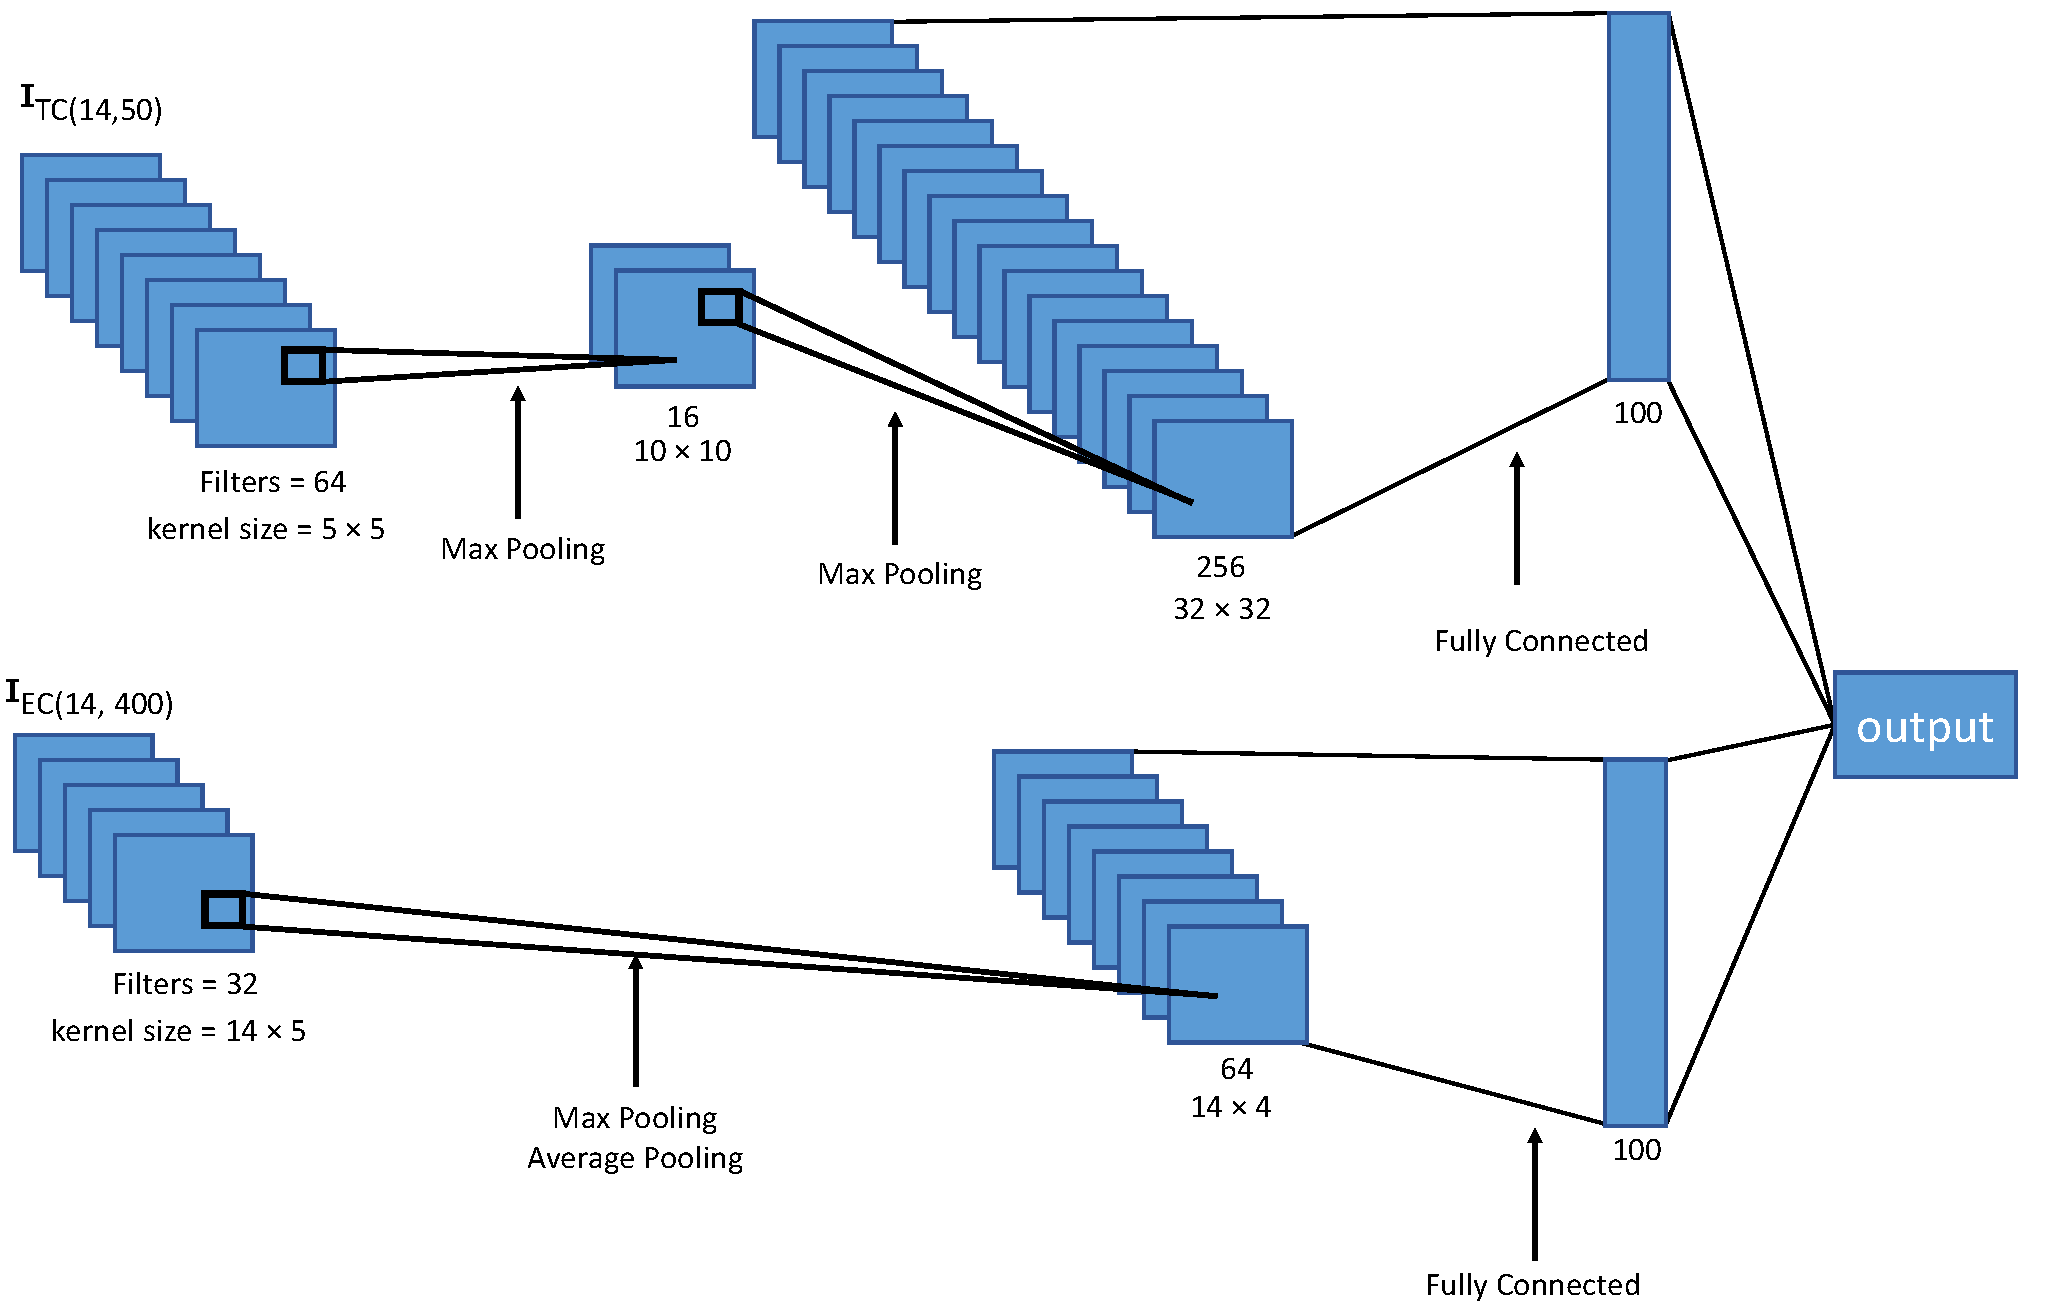
\includegraphics[width=0.9\textwidth]{1111modelFinalVisualize.pdf} \caption{Architecture of the convolutional neural network model. The type-centric model (top) and the bottom-centric model (bottom) are combined in a single network.}
	\label{proposeModel}
\end{figure*}
